\chapter{Технологический раздел}
\label{cha:technological}

    В данном разделе представлены требования к ПО, средства, использованные в процессе разработки для реализации задачи, а также листинг кода программы. Кроме того описан пользовательский интерфейс и показаны результаты тестирования.

    \section{Требования к ПО}
    \par На рисунке (\ref{schema:idef}) представлена IDEF0 диаграмма реализуемой задачи.
    \begin{figure}[h!]
            \centering
            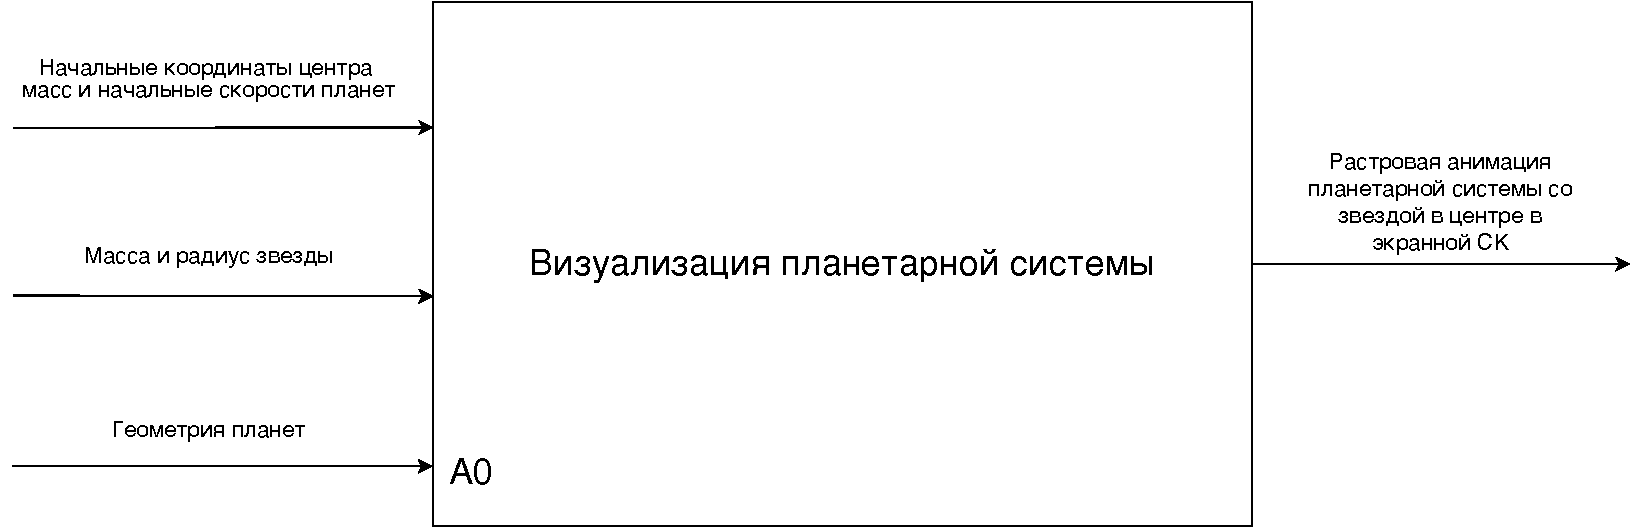
\includegraphics[scale=0.6]{inc/idef.pdf}
            \caption{IDEF0 диаграмма разрабатываемого ПО}
            \label{schema:idef}
        \end{figure}\clearpage
    \par Программа должна предоставлять доступ к следующему функционалу:
    \begin{enumerate}
            \item добавление звезды на сцену;
            \item добавление планет на сцену;
            \item пауза, старт и сброс анимации;
            \item перемещение камеры на сцене.
        \end{enumerate}
    \par К программе предъявляются следующие требования:
    \begin{enumerate}
            \item программа должна давать отклик на действия пользователя за минимальное время;
            \item программа должна корректно реагировать на любые действия пользователя.
        \end{enumerate}

    \section{Средства реализации разработанного ПО}
        Для реализации был использован язык C++, так как он предоставляет весь необходимый функционал для решения поставленной задачи, а также для него существует фреймворк QT со встроенным графическим редактором QT Design, который позволит создать пользовательский интерфейс.

    \section{Листинг программы}
        В приведенных ниже листингах представлены следующие реализации: 
        \begin{enumerate}
            \item модифицированный алгоритм $Z$-буфера (листинг \ref{lst:Zb});
            \item алгоритм простой закраски (листинг \ref{lst:P_z});
            \item алгоритм построения полигональной сетки (листинг \ref{lst:Pol}).
        \end{enumerate}
        \par \text{           }
        \begin{lstlisting}[language=C++, label=lst:Zb, caption=Модифицированный алгоритм Z-буфера]
void myGraphicsView::DrawSystem()
{
    scene->clear();
    DrawStars();

    int z[MAX_OBJECTS_SIZE][Z_MATRIX_ROW_SIZE];
    for (auto i = 0; i < objects.size(); i++)
    {
        z[i][0] = (objects[i]).GetCenter().GetZ();
        z[i][1] = i;
    }

    if (objects.size() > 0)
    {
        for (auto i = 0; i < objects.size() - 1; i++)
            for (auto j = 0; j < objects.size() - i - 1; j++)
                if (z[j][0] > z[j + 1][0])
                {
                    std::swap(z[j][0], z[j + 1][0]);
                    std::swap(z[j][1], z[j + 1][1]);
                }
    }
    int i = 0;

    while (i < objects.size() && z[i][0] < star[0].GetCenter().GetZ())
        DrawPlanet(objects[z[i++][1]]);
    DrawStar();
    while (i < objects.size())
        DrawPlanet(objects[z[i++][1]]);
}

//Пример отрисовки Звезды
void myGraphicsView::DrawStar()
{
    Edge* net = star[0].GetEdges();
    Point* points = star[0].GetPoints();
    int n = star[0].GetNetNodesParam();
    int cz = star[0].GetCenter().GetZ();
    Point p1, p2, p3;
    double t = star[0].GetCenter().GetZ() / Z_K;

    std::vector<Point> orbit = star[0].GetOrbitNum();
    int no = orbit.size();
    int j;
    for (int i = 0; i < no - 1; i++)
    {
        DrawLine(orbit[i], orbit[i+1]);
    }
    for (int i = 0; i < star[0].GetEdgesNum(); i++)
    {
        p1 = points[net[i].GetP1()];
        p2 = points[net[i].GetP2()];
        p3 = points[net[i].GetP3()];
        if (p1.GetZ() >= cz || p2.GetZ() >= cz || p3.GetZ() >= cz)
            DrawPolygon(p1, p2, p3, 1 + t, star[0].GetCenter());
    }
}
    \end{lstlisting}
    \par \text{  }
    \begin{lstlisting}[language=C++, label=lst:P_z, caption=Алгоритм простой закраски]
void PlanetA::CalcIntensities(std::vector<Point> lights)
{
    Edge* edges = GetEdges();
    Point* points = GetPoints();
    int n = GetNetNodesParam();

    Vector *normals = new Vector[GetEdgesNum()];
    Point a, b, c;
    Vector ab, ac, ra;
    int I_0 = 1, I;
    double cos_lamb, cos_r;
    double len_n, len_a, len_r;
    double sn, sr;

    Point center = GetCenter();

    for (int i = 0; i < GetEdgesNum(); i++)
    {
        intensities[i] = 0;
        for (int j = 0; j < GetEdgesNum(); j++)
        {
            a = points[edges[i].GetP1()];
            b = points[edges[i].GetP2()];
            c = points[edges[i].GetP3()];

            ab.Set(a, b);
            ac.Set(a, c);
            normals[i] = ab.VectProd(ac);

            ra.Set(a, center);
            len_r = ra.GetLen();
            sr = normals[i].ScalarProd(ra);
            len_n = normals[i].GetLen();
            len_a = a.GetDistance(lights[j]);

            cos_r = sr / len_r / len_n;
            if (cos_r > 0)
                normals[i].Neg();

            sn = normals[i].ScalarProd(Vector(a, lights[j]));
            cos_lamb = sn / len_n / len_a;

            intensities[i] += I_0 * cos_lamb;
        }
    }
    delete [] normals;
}
        \end{lstlisting}

        \begin{lstlisting}[language=C++, label=lst:Pol, caption=Алгоритм построения полигональной сетки]
void Object::CreateNet()
{
    CreatePoints();
    CreateEdges();
}

void Object::CreatePoints()
{
    points = new Point [GetPointsNum()];
    int k = 0;
    int r = radius_a;
    int cx = center.GetX(); int cy = center.GetY(); int cz = center.GetZ();

    points[k++] = Point(cx - r, cy, cz);

    int step_degree = 90 / (net_nodes_param + 1);
    double radians, a, b, c;
    for (int i = 1; i <= net_nodes_param; i++)
    {
        radians = (90 - step_degree * i) * M_PI / 180;
        if (type == 0)
        {
            a = sqrt(2 * r * r * (1 - cos(radians)));
            b = sin(radians) * r;
            c = sqrt(a * a - b * b);
            points[k++] = Point(cx - b, cy + r - c, cz);
        }
        else if (type == 1)
        {
            int r_tmp = round(sqrt((radius_a*radius_a*radius_b*radius_b) / (cos(radians)*cos(radians)
            *radius_a*radius_a+sin(radians)*sin(radians)*radius_b*radius_b)));
            a = sqrt(2 * r_tmp * r_tmp * (1 - cos(radians)));
            b = sin(radians) * r_tmp;
            c = sqrt(a * a - b * b);
            points[k++] = Point(cx - b, cy + radius_a - c, cz);
        }
    }
    points[k++] = Point(cx, cy + r, cz);

    for (int i = 0; i <= net_nodes_param; i++)
    {
        points[k++] = Point(2 * cx - points[net_nodes_param - i].GetX(),
                          points[net_nodes_param - i].GetY(),
                          points[net_nodes_param - i].GetZ());
    }
}

void Object::CreateEdges()
{
    int n = 3 + net_nodes_param * 2;
    int m = 2 + net_nodes_param * 2 * 2;

    Edge cur_edges[m];
    edges = new Edge[GetEdgesNum()];

    int j = 0;
    int top_set[n];
    int bottom_set[n];
    double step_degree = 90 / (net_nodes_param + 1);
    int k = n;
    int cur, right, left;

    for (int i = 0; i < n; i++)
    {
        top_set[i] = i;
    }

    int s = n;

    for (double degree = step_degree; degree <= 360; degree += step_degree)
    {
        for (int i = 1; i < n - 1; i++)
        {
            Point temp = points[i];
            points[s++] = temp.RotateX(degree, center);
        }
        for (int i = 0; i < n - 2; i++)
        {
            bottom_set[i] = k + i;
        }
        for (int i = 0; i < m; i++)
        {
            cur_edges[i] = Edge();
        }

        cur_edges[0].Append(top_set[0]);
        cur_edges[n - 2].Append(top_set[n - 1]);

        for (int i = 1; i < n - 1; i++)
        {
            cur_edges[i - 1].Append(top_set[i]);
            cur_edges[i].Append(top_set[i]);
        }

        for (int i = 2; i < n - 1; i++)
        {
            cur_edges[n - 1 + i - 2].Append(top_set[i]);
        }
        for (int i = 0; i < n - 2; i++)
        {
            cur = (n + i) % (n - 1);
            right = (n - 1) + i;
            left = right - 1;
            if (cur == 1)
            {
                left = 0;
            }
            cur_edges[cur].Append(bottom_set[i]);
            cur_edges[left].Append(bottom_set[i]);
            if (cur != n - 2)
            {
                cur_edges[right].Append(bottom_set[i]);
            }
        }
        for (int i = j; i < j + m; i++)
        {
            edges[i] = cur_edges[i % m];
        }
        j += m;
        top_set[0] = 0;
        top_set[n - 1] = n - 1;
        for (int i = 0; i < n - 2; i++)
        {
            top_set[i + 1] = bottom_set[i];
        }
        k += n - 2;
    }

    for (int i = 0; i < n - 2; i++)
    {
        bottom_set[i] = top_set[i + 1];
    }
    for (int i = 0; i < n; i++)
    {
        top_set[i] = i;
    }
    for (int i = 0; i < m; i++)
    {
        cur_edges[i] = Edge();
    }

    cur_edges[0].Append(top_set[0]);
    cur_edges[n - 2].Append(top_set[n - 1]);

    for (int i = 1; i < n - 1; i++)
    {
        cur_edges[i - 1].Append(top_set[i]);
        cur_edges[i].Append(top_set[i]);
    }

    for (int i = 2; i < n - 1; i++)
    {
        cur_edges[n - 1 + i - 2].Append(top_set[i]);
    }
    for (int i = 0; i < n - 2; i++)
    {
        cur = (n + i) % (n - 1);
        right = (n - 1) + i;
        left = right - 1;
        if (cur == 1)
        {
            left = 0;
        }
        cur_edges[cur].Append(bottom_set[i]);
        cur_edges[left].Append(bottom_set[i]);
        if (cur != n - 2)
        {
            cur_edges[right].Append(bottom_set[i]);
        }
    }
    for (int i = j; i < j + m; i++)
    {
        edges[i] = cur_edges[i % m];
    }

}
        \end{lstlisting}

    \section{Описание интерфейса программы}
    \par Программа запускается с помощью среды разработки Qt Creator: необходимо только нажать на кнопку сборки и запуска в левом нижнем углу.
    \par Существует альтернативный способ запуска с помощью CMake и использования следующей команды: ./build\_release.sh (листинг \ref{lst:build})
    \begin{lstlisting}[language=C++, label=lst:build, caption=Release сборка программы для терминала]
#!/bin/bash

cd .. && rm -rf build && cd planet_system

mkdir ../build && cd ../build

cmake -DCMAKE_BUILD_TYPE=Release ../planet_system

cmake --build .

./planet_system
    \end{lstlisting}
    \par На рисунках (\ref{img:PO}, \ref{img:PO_1}, \ref{img:PO_2}) представлен интерфейс программного продукта. Три верхние кнопки используются для остановки, запуска и сброса анимации. Следующие два окна для ввода исходных данных для моделирования движения. Затем две кнопки реализуют масштабирование относительно центра Звезды: вперед и назад. Последняя кнопка отвечает за завершение приложения.

    \begin{figure}[h!]
            \centering
            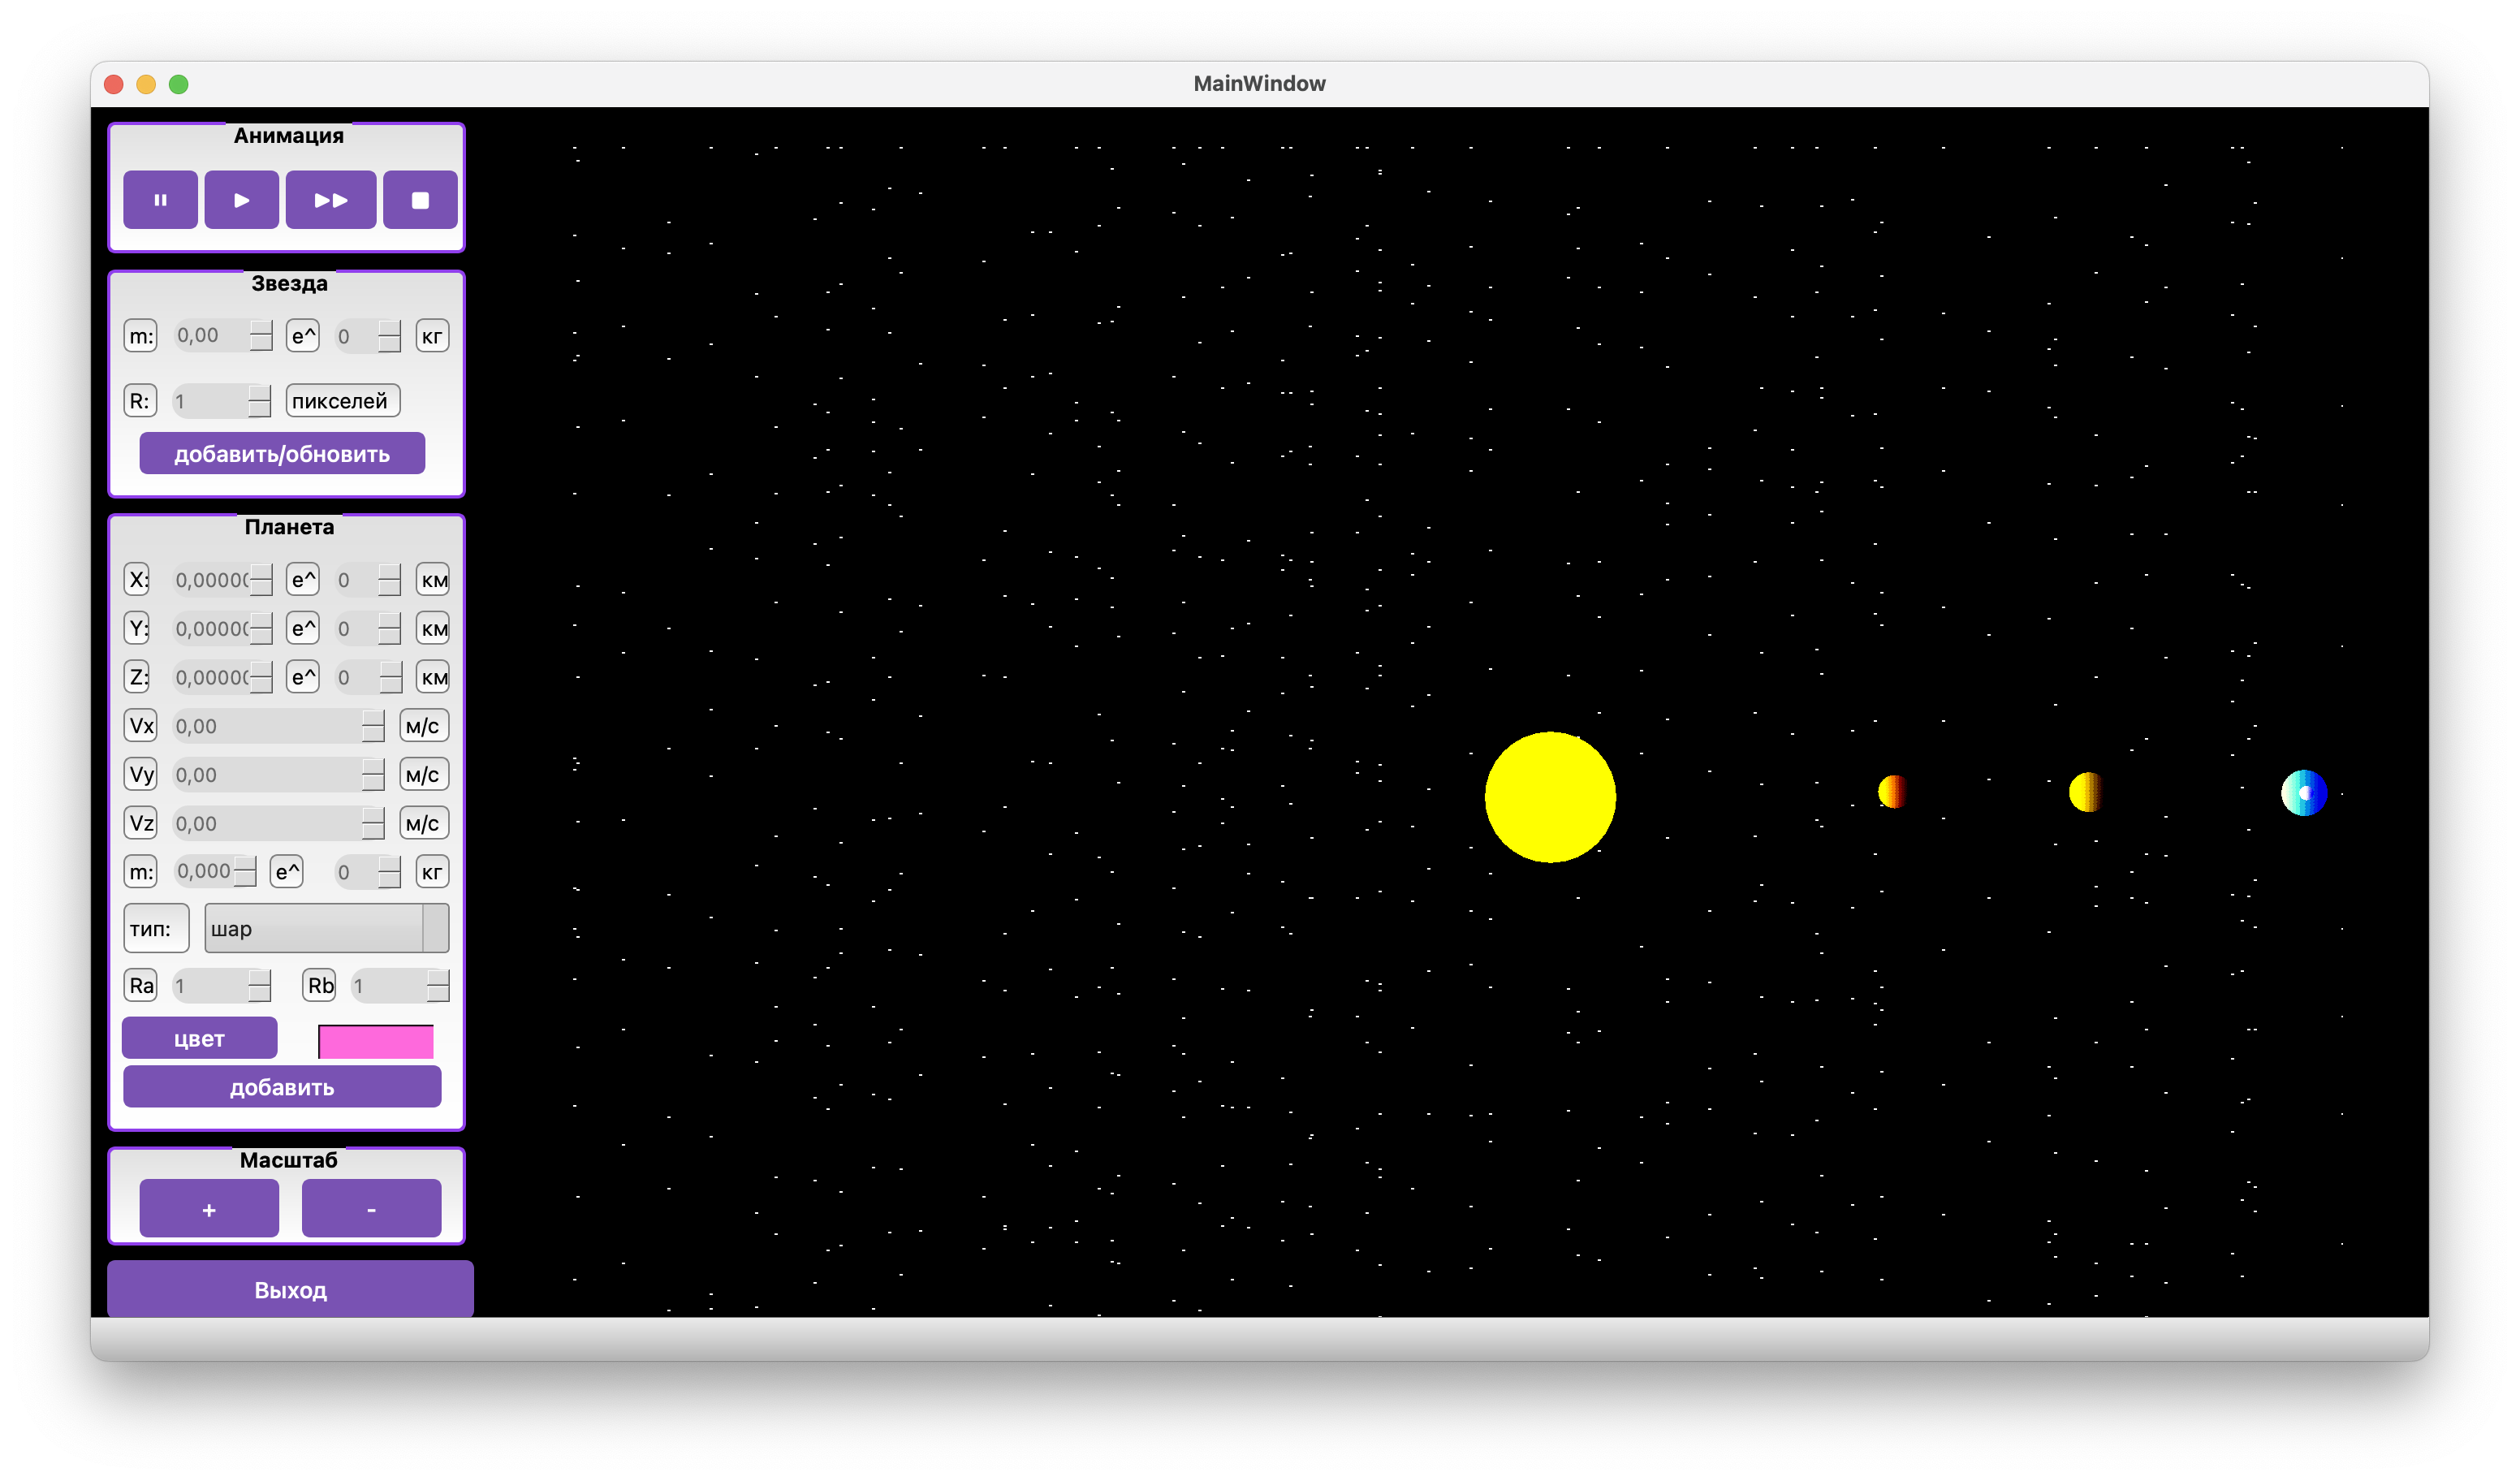
\includegraphics[scale=0.35]{inc/PO.png}
            \caption{Интерфейс ПО}
            \label{img:PO}
    \end{figure}\clearpage

    \begin{figure}[h!]
            \centering
            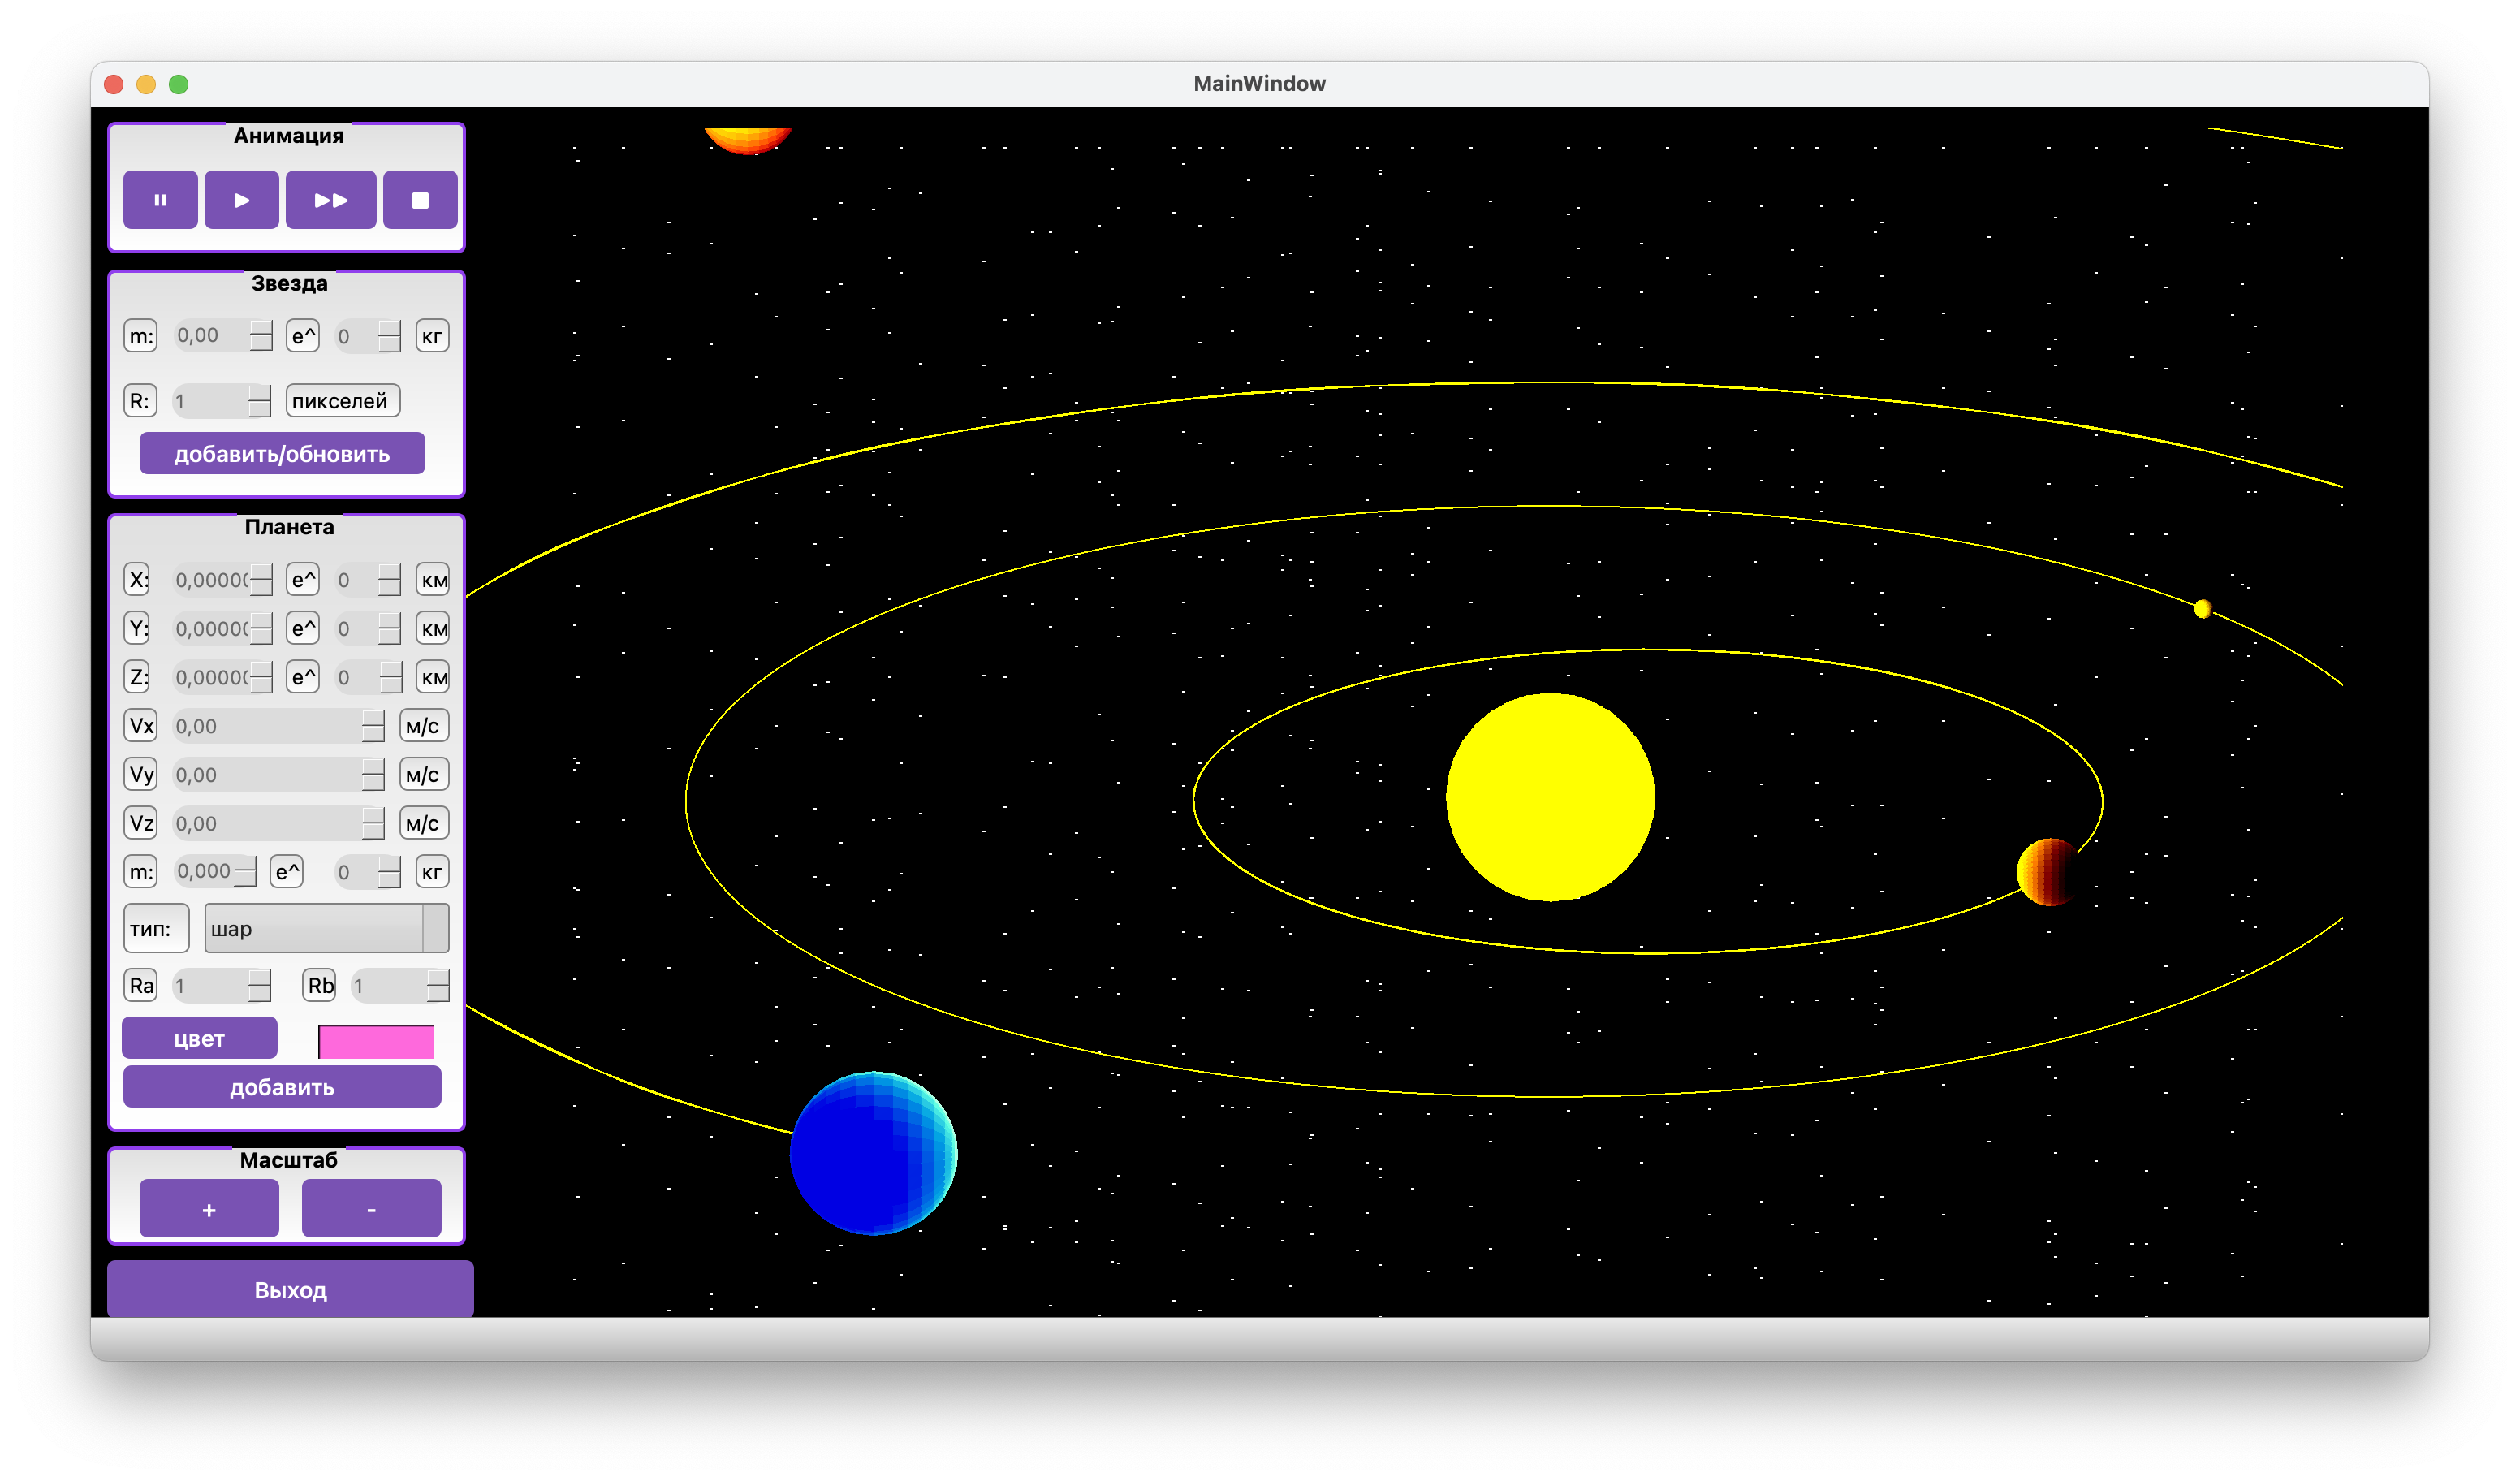
\includegraphics[scale=0.35]{inc/PO_1.png}
            \caption{Интерфейс ПО}
            \label{img:PO_1}
    \end{figure}\clearpage

    \begin{figure}[h!]
            \centering
            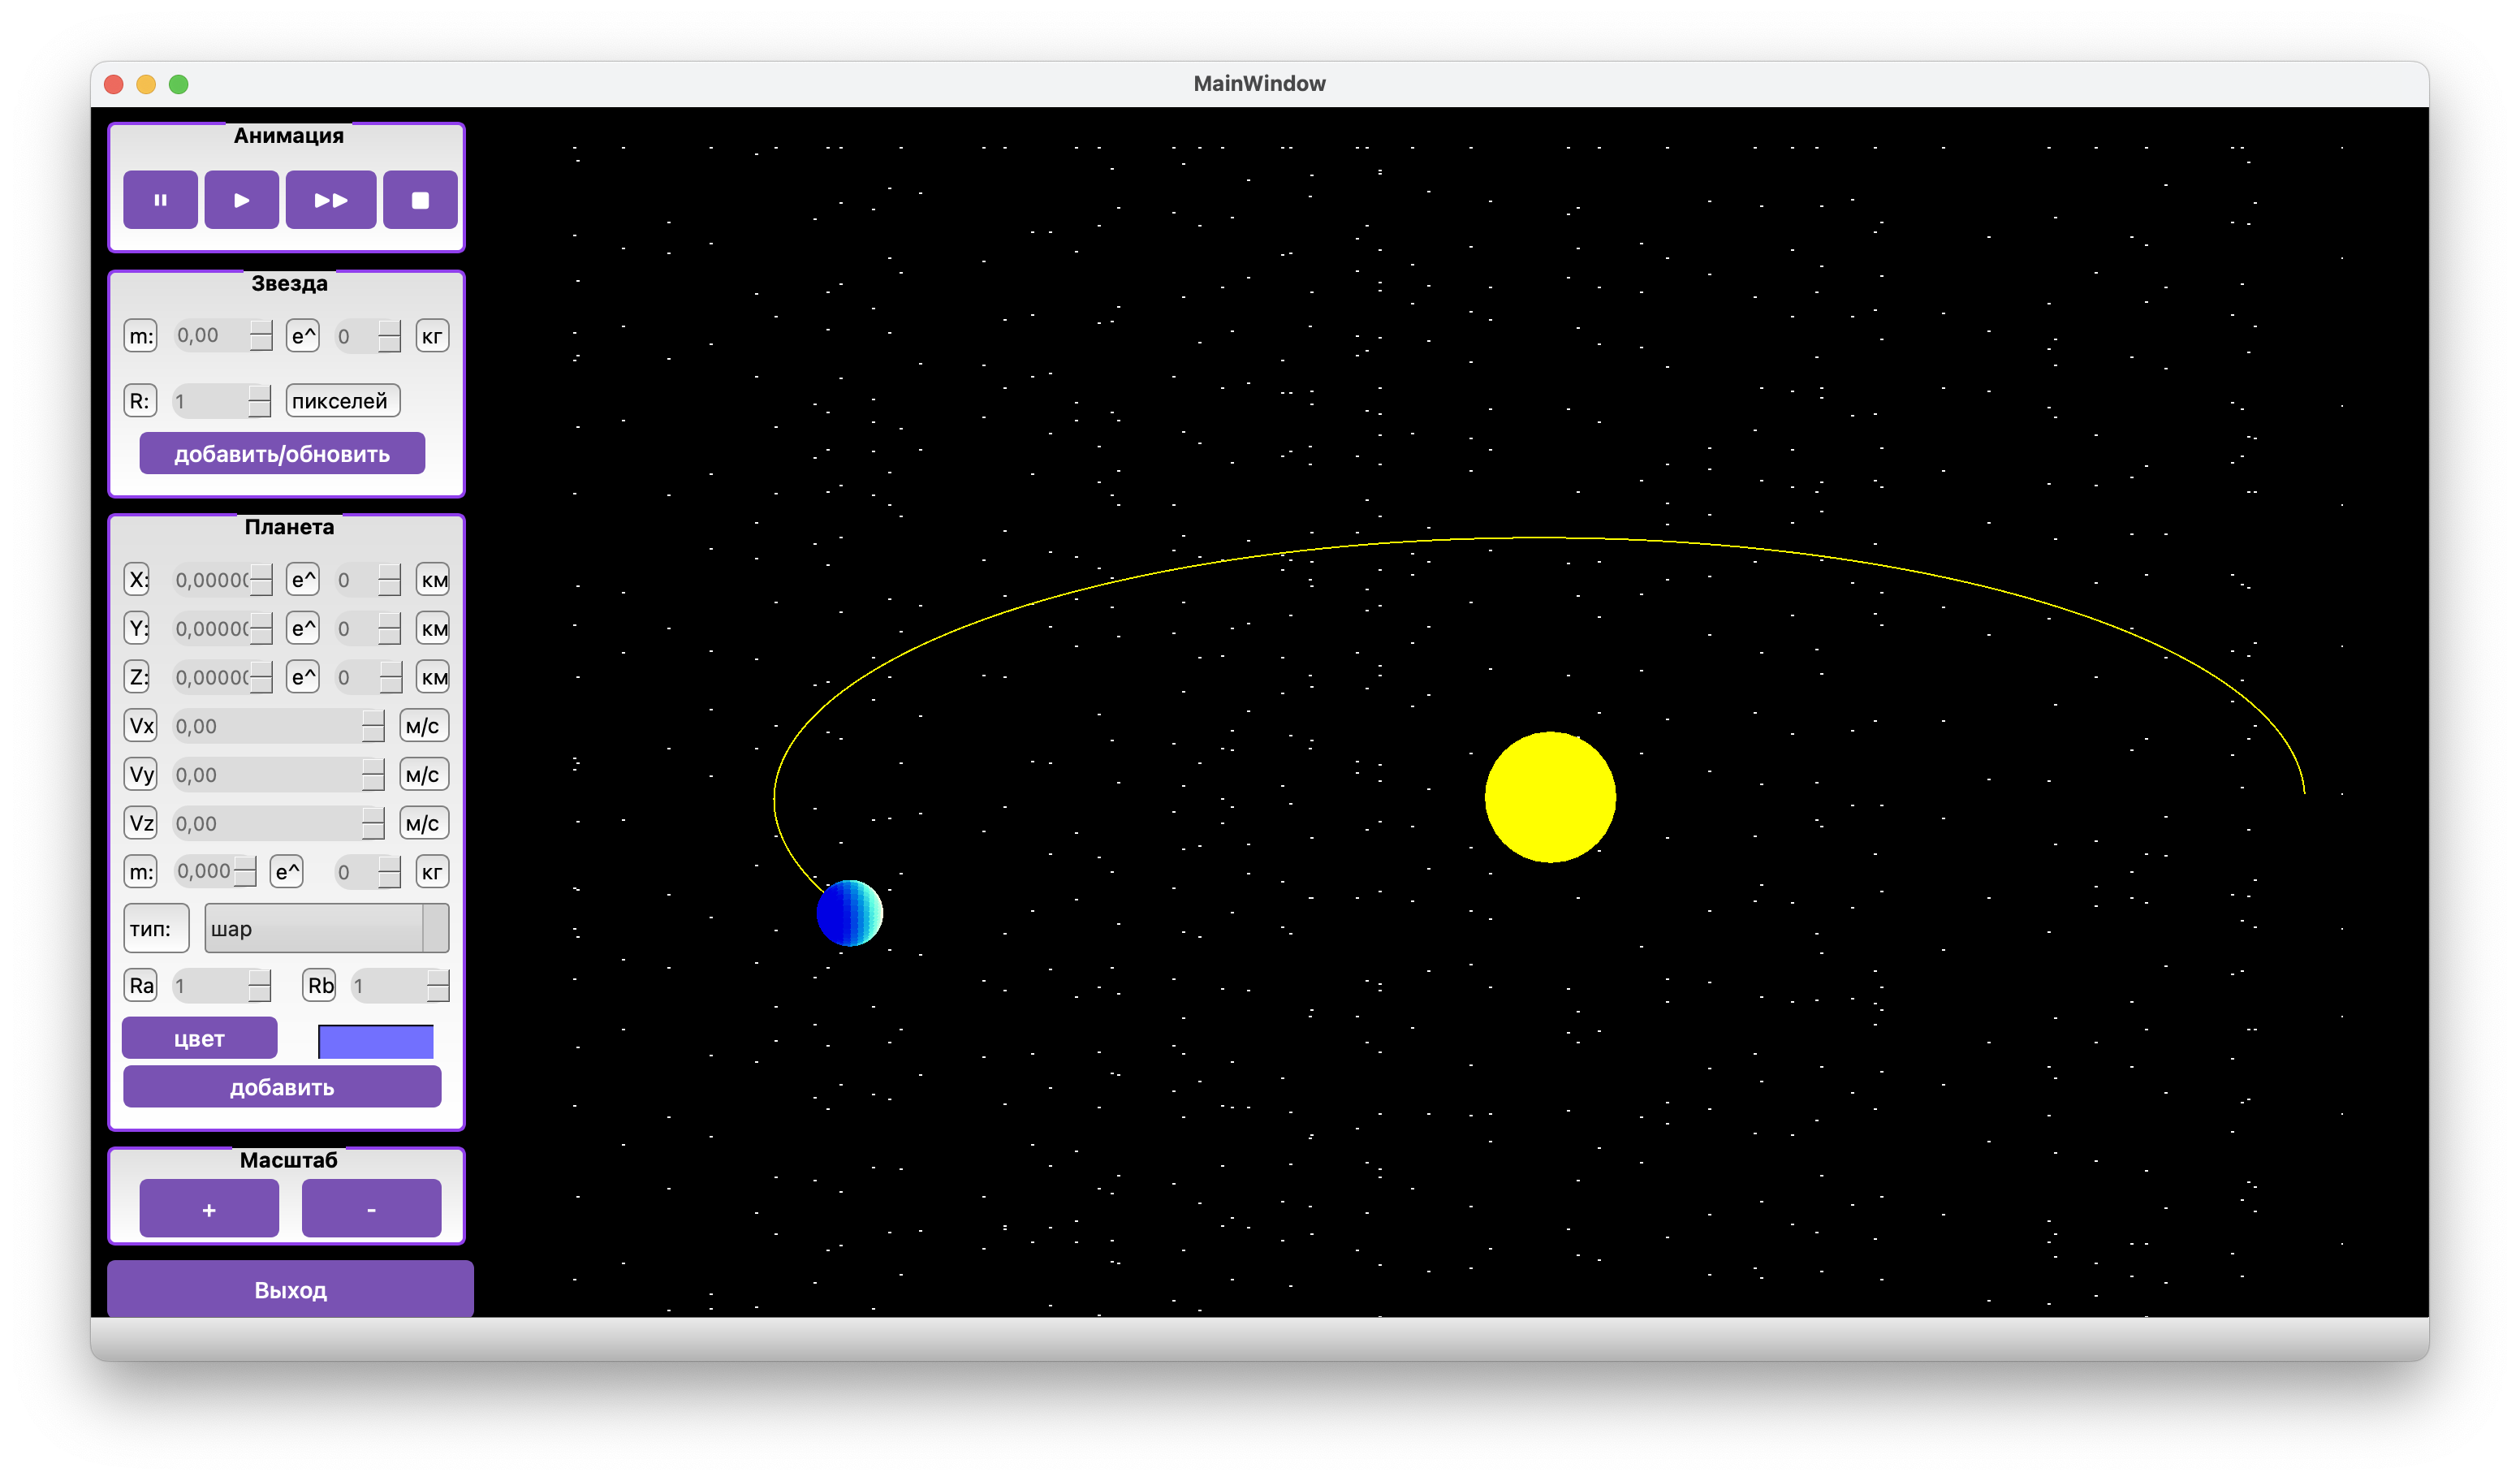
\includegraphics[scale=0.35]{inc/PO_2.png}
            \caption{Интерфейс ПО}
            \label{img:PO_2}
    \end{figure}\clearpage

    \section{Модульное тестирование}
    \par Было произведено тестирование одного из модулей программы с помощью 
библиотеки testlib и фреймворка Qt Test.
\par Для тестирования был выбран модуль myGraphicsView, из которого были выбраны 
функциы CalcNewPos, AddNewPlanet и UpdateStar. Создан класс Test, наследуемый от класса 
QObject. В публичном слоте находится конструктор класса, а в приватном —
непосредственно создаваемые тесты. [\ref{bib:9}]
\begin{lstlisting}[label=some-code,caption= Класс TestG для тестирования модуля Vector]
class TestG : public QObject {
    Q_OBJECT
public:
    explicit TestG(QObject* parent = nullptr, myGraphicsView* g = nullptr);

private:
    myGraphicsView* m_g;
private slots:
    void test_g_01();
    void test_g_02();
    void test_g_03();
    void test_g_04();
};
\end{lstlisting}
\par Таким образом, чтобы добавить новый тест, достаточно создать новый 
приватный слот. В данном случае добавление теста будет выглядеть следующим 
образом:
\begin{lstlisting}[label=some-code,caption= пример добавления нового модульного теста]
private slots:
    void test_g_01();
    void test_g_02();
    void test_g_03();
    void test_g_04();
\end{lstlisting}
\par Ниже приведен листинг реализации конкретного теста проверки рассчета нормали к заданной поверхности. Проверка корректности полученного результата производится с помощью макросов фреймворка Qt Test. В данном примере используется макрос 
QCOMPARE, сравнивающий ожидаемое значение с полученным.
\begin{lstlisting}[label=some-code,caption= реализация модульного теста test\_g\_03]
void TestG::test_g_03()
{
    Star s (Point(600,400,5), 10, 0, 2e30) ;
    Point * test = s.GetPoints();
    std::vector<Point> test_tmp = {Point(590, 400, 5),
                                   Point(600, 410, 5),
                                   Point(610, 400, 5),
                                   Point(600, 400, 15),
                                   Point(600, 390, 5),
                                   Point(600, 400, -5),
                                   Point(600, 410, 5),
                                   Point(0, 0, 0),
                                   Point(0, 0, 0),
                                   Point(0, 0, 0),
                                   Point(0, 0, 0)};
    for(int i = 0; i < s.GetPointsNum(); i++)
    {
        QCOMPARE(qFuzzyCompare(test[i].GetX(), test_tmp[i].GetX()), true);
        QCOMPARE(qFuzzyCompare(test[i].GetY(), test_tmp[i].GetY()), true);
        QCOMPARE(qFuzzyCompare(test[i].GetZ(), test_tmp[i].GetZ()), true);
    }
}
\end{lstlisting}
\par Функция qFuzzyCompare используется для корректного сравнения чисел с 
плавающей точкой, так как QCOMPARE сравнивает числа с помощью оператора 
«==». Такое сравнение не используется для чисел с плавающей точкой, но 
подходит для сравнения значений типа bool, что и показано в приведенном 
примере.
\section{Реализация управления из командной строки}
\par Для автоматизации работы программы и использования сценария было 
необходимо реализовать передачу в программу аргументов командной строки и 
их распознавание самой программой. Для этого была использована библиотека 
getopt [\ref{bib:10}], позволяющая выполнить «сканирование» аргументов командной 
строки и их обработку. Конкретно была использована одноименная функция 
getopt, которая последовательно перебирает переданные параметры в программу 
в соответствии с заданной строкой параметров, содержащей имена параметров и 
признак наличия передаваемого значения («:»).
Перечень используемых параметров:
\begin{enumerate}
\item Флаг «-t» — указание программе о том, что нужно провести замер времени и вызвать python скрипт, который сгенерирует графики;
\item Флаг «-e» — указание программе о том, что проводится модульное тестирование;
\item Флаг «-i n» — указание программе о том, что нужно отрисовать n сцен и сохранить их в формате $png$.
\end{enumerate}
\begin{lstlisting}[label=some-code,caption= пример вызова программы для создания изображений ]
#!/bin/bash

./planet_system -i 20 
\end{lstlisting}

	\section{Выводы из технологического раздела}
	\par В данном разделе были рассмотрены средства реализации, описаны основные моменты программной реализации, рассмотрен интерфейс программного продукта, методы тестирования и управления из командной строки.
    	
\newpage